\thispagestyle{empty}

\chapter{Real-Time Localization System}
\thispagestyle{empty}
\label{cpt:localization}

This chapter focuses on the real-time LiDAR localization system. With the foundational point cloud map established, we can match current laser scan data with the map to determine the vehicle's position, which is then fused with IMU and other sensor data using filters \cite{Wang2017}. However, point cloud localization doesn't directly provide physical world coordinates like RTK does - it first requires an approximate initial position to guide the point cloud registration algorithm toward convergence. Consequently, point cloud localization presents some unique logical challenges in practical applications. Using the point cloud map constructed in the previous chapter, this chapter demonstrates the implementation of point cloud localization and presents a real-time localization solution based on a Kalman filter.

\includepdf[width=\textwidth]{art/ch10.pdf}

\section{Design Scheme for Point Cloud Fusion Localization}  
Before designing the overall algorithm flow, let us first examine the characteristics of various sensor inputs.

Compared to traditional integrated navigation systems, high-precision localization for autonomous vehicles primarily incorporates an additional input source: LiDAR-based localization. Traditional RTK-IMU integrated navigation systems are less suitable for scenarios like campuses due to the inherent signal quality limitations of RTK. As readers may observe from the NCLT dataset, RTK signals often exhibit instability—such as jitter or dropout—in many areas. On the other hand, the point cloud map constructed in the previous chapter provides an excellent representation of the 3D structure of static environments. Most large-scale scenes, such as buildings, do not change frequently, making point cloud localization a reliable positioning source. Previous chapters of this book have extensively discussed methods for registering scan point clouds with map point clouds. This chapter will employ the NDT method for registration and ultimately integrate the results into a Kalman filter.

\begin{figure}[!htp]  
	\centering  
	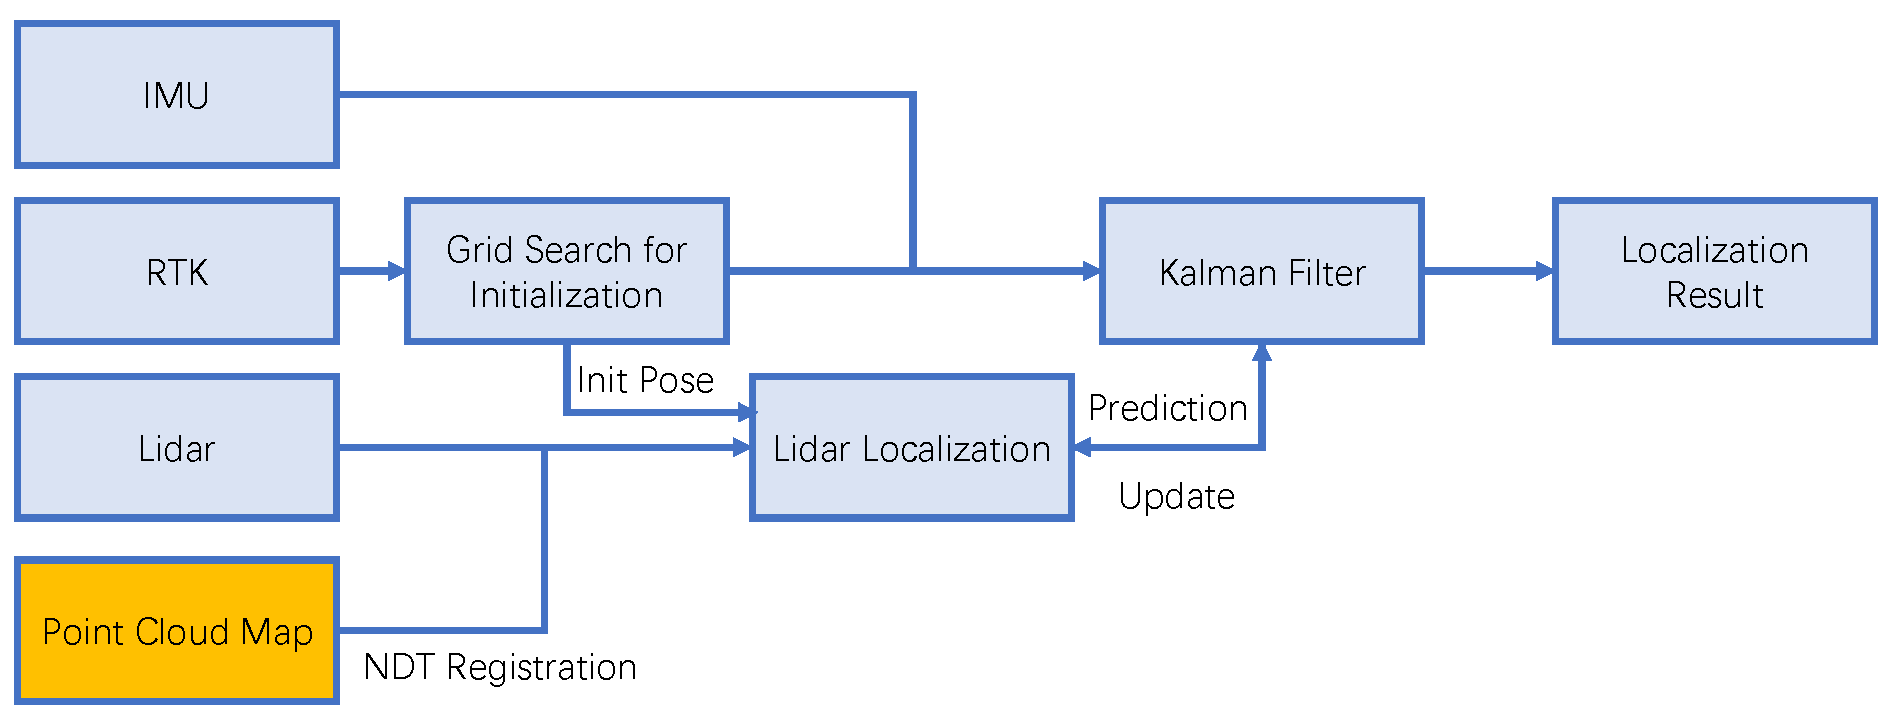
\includegraphics[width=0.8\textwidth]{resources/localization/framework}  
	\caption{Algorithm framework for point cloud fusion localization}  
	\label{fig:localization-framework}  
\end{figure}  

From a fusion perspective, point cloud fusion localization can adopt either an error-state Kalman filter (similar to traditional integrated navigation) or pose graph optimization (like modern SLAM systems). Generally, the Kalman filter approach is simpler to design and implement, often yielding smoother results. However, it may converge to incorrect solutions, leading to localization drift that is difficult to correct. In contrast, graph optimization methods facilitate the detection of discrepancies between various factors and the estimated state, enabling logical handling of anomalies—though ensuring smoothness in localization is more challenging (unless manual marginalization, as in Chapter~\ref{cpt:ins}, is performed, or optimization libraries like GTSAM with built-in marginalization are used).  

First, let us examine the overall algorithm framework (see Fig.~\ref{fig:localization-framework}). This chapter demonstrates a Kalman filter-based localization solution. Since the principles of the Kalman filter have already been detailed in Chapter~\ref{cpt:ins}, the focus here will be on the fusion of point cloud localization with the Kalman filter.  

Point cloud localization requires an initial vehicle position for search, so we design an initialization procedure. When the filter has not yet computed its position, the first valid RTK signal is used to constrain the search range for point cloud localization. Additionally, since the RTK data in the NCLT dataset lacks attitude information, a grid search is employed to determine the vehicle's orientation. Once the Kalman filter converges, its predicted value serves as the initial guess for point cloud registration\footnote{Alternatively, the point cloud localization could predict the next LiDAR pose based on historical poses, improving system decoupling and simplifying debugging.}.  

At the point cloud localization level, we use the partitioned point clouds from the previous chapter. Since the point clouds were divided into 100m×100m grid cells earlier, this chapter loads a 3×3 grid (nine cells) around the vehicle. To prevent frequent loading/unloading when the vehicle moves near grid boundaries, an unloading threshold (set to three cells in our implementation) is applied—only cells beyond this range are unloaded.

\section{Algorithm Implementation}  
Now we proceed to implement the algorithm described earlier. The code implementation in this chapter reuses portions of the filter from Chapter~\ref{cpt:ins} and the IMU processing code from Chapter~\ref{cpt:tightly-lio}.  

\subsection{RTK Initialization Search}  
Following the algorithm flow outlined previously, the system cannot perform point cloud localization until it receives the first valid RTK signal, as the vehicle's position in the map is unknown. Upon receiving the first valid RTK signal, we conduct a \textbf{grid search} around it. Our designed search process primarily determines the vehicle's initial heading angle by employing a multi-resolution matching method similar to that used in loop detection (Chapter~\ref{cpt:tightly-lio}).  

\begin{lstlisting}[language=c++,caption=/ch10/fusion.cc]  
bool Fusion::SearchRTK() {  
	// Since RTK lacks attitude, we must search within an angular range  
	std::vector<GridSearchResult> search_poses;  
	LoadMap(last_gnss_->utm_pose_);  
	
	/// RTK provides no orientation, so we scan angles at fixed intervals  
	double grid_ang_range = 360.0, grid_ang_step = 10;  // Angular search range and step  
	for (double ang = 0; ang < grid_ang_range; ang += grid_ang_step) {  
		SE3 pose(SO3::rotZ(ang * math::kDEG2RAD), Vec3d(0, 0, 0) + last_gnss_->utm_pose_.translation());  
		GridSearchResult gr;  
		gr.pose_ = pose;  
		search_poses.emplace_back(gr);  
	}  
	
	LOG(INFO) << "grid search poses: " << search_poses.size();  
	std::for_each(std::execution::par_unseq, search_poses.begin(), search_poses.end(),  
	[this](GridSearchResult& gr) { AlignForGrid(gr); });  
	
	// Select the best-matching result  
	auto max_ele = std::max_element(search_poses.begin(), search_poses.end(),  
	[](const auto& g1, const auto& g2) { return g1.score_ < g2.score_; });  
	LOG(INFO) << "max score: " << max_ele->score_ << ", pose: \n" << max_ele->result_pose_.matrix();  
	if (max_ele->score_ > rtk_search_min_score_) {  
		LOG(INFO) << "Initialization succeeded, score: " << max_ele->score_ << ">" << rtk_search_min_score_;  
		status_ = Status::WORKING;  
		
		/// Reset filter state  
		auto state = eskf_.GetNominalState();  
		state.R_ = max_ele->result_pose_.so3();  
		state.p_ = max_ele->result_pose_.translation();  
		state.v_.setZero();  
		eskf_.SetX(state, eskf_.GetGravity());  
		
		ESKFD::Mat18T cov;  
		cov = ESKFD::Mat18T::Identity() * 1e-4;  
		cov.block<12, 12>(6, 6) = Eigen::Matrix<double, 12, 12>::Identity() * 1e-6;  
		eskf_.SetCov(cov);  
		
		return true;  
	}  
	
	init_has_failed_ = true;  
	last_searched_pos_ = last_gnss_->utm_pose_;  
	return false;  
}  

void Fusion::AlignForGrid(sad::Fusion::GridSearchResult& gr) {  
	/// Multi-resolution NDT  
	pcl::NormalDistributionsTransform<PointType, PointType> ndt;  
	ndt.setTransformationEpsilon(0.05);  
	ndt.setStepSize(0.7);  
	ndt.setMaximumIterations(40);  
	
	ndt.setInputSource(current_scan_);  
	auto map = ref_cloud_;  
	
	CloudPtr output(new PointCloudType);  
	std::vector<double> res{10.0, 5.0, 4.0, 3.0};  
	Mat4f T = gr.pose_.matrix().cast<float>();  
	for (auto& r : res) {  
		auto rough_map = VoxelCloud(map, r * 0.1);  
		ndt.setInputTarget(rough_map);  
		ndt.setResolution(r);  
		ndt.align(*output, T);  
		T = ndt.getFinalTransformation();  
	}  
	
	gr.score_ = ndt.getTransformationProbability();  
	gr.result_pose_ = Mat4ToSE3(ndt.getFinalTransformation());  
}  
\end{lstlisting}

\section{Algorithm Implementation}
We concurrently invoke multi-resolution NDT searches to determine the vehicle's initial orientation. If the maximum matching score from these registration results exceeds a preset threshold, we consider the initialization successful. Upon successful RTK initialization, the fusion system transitions to normal operation mode. The code framework here resembles the LIO system described earlier. We retain the point cloud deskewing and IMU-LiDAR message synchronization components while replacing the original LIO registration with map matching:

\begin{lstlisting}[language=c++,caption=/ch10/fusion.cc]
	void Fusion::ProcessMeasurements(const MeasureGroup& meas) {
		measures_ = meas;
		
		if (imu_need_init_) {
			TryInitIMU();
			return;
		}
		
		/// The following three steps remain consistent with LIO, 
		/// except the map matching is now handled by the align function
		if (status_ == Status::WORKING) {
			Predict();
			Undistort();
		} else {
			scan_undistort_ = measures_.lidar_;
		}
		
		Align();
	}
	
	void Fusion::Align() {
		FullCloudPtr scan_undistort_trans(new FullPointCloudType);
		pcl::transformPointCloud(*scan_undistort_, *scan_undistort_trans, TIL_.matrix());
		scan_undistort_ = scan_undistort_trans;
		current_scan_ = ConvertToCloud<FullPointType>(scan_undistort_);
		current_scan_ = VoxelCloud(current_scan_, 0.5);
		
		if (status_ == Status::WAITING_FOR_RTK) {
			// If recent RTK signal exists, attempt initialization
			if (last_gnss_ != nullptr) {
				if (SearchRTK()) {
					status_ == Status::WORKING;
					ui_->UpdateScan(current_scan_, eskf_.GetNominalSE3());
					ui_->UpdateNavState(eskf_.GetNominalState());
				}
			}
		} else {
			LidarLocalization();
			ui_->UpdateScan(current_scan_, eskf_.GetNominalSE3());
			ui_->UpdateNavState(eskf_.GetNominalState());
		}
	}
\end{lstlisting}

At the LiDAR registration level, we load point clouds near the predicted pose and perform NDT registration:

\begin{lstlisting}[language=c++,caption=/ch10/fusion.cc]
	bool Fusion::LidarLocalization() {
		SE3 pred = eskf_.GetNominalSE3();
		LoadMap(pred);
		
		ndt_.setInputCloud(current_scan_);
		CloudPtr output(new PointCloudType);
		ndt_.align(*output, pred.matrix().cast<float>());
		
		SE3 pose = Mat4ToSE3(ndt_.getFinalTransformation());
		eskf_.ObserveSE3(pose, 1e-1, 1e-2);
		
		LOG(INFO) << "lidar loc score: " << ndt_.getTransformationProbability();
		
		return true;
	}
\end{lstlisting}

The LoadMap function loads/unloads necessary map blocks based on the given pose:

\begin{lstlisting}[language=c++,caption=/ch10/fusion.cc]
	void Fusion::LoadMap(const SE3& pose) {
		int gx = int((pose.translation().x() - 50.0) / 100);
		int gy = int((pose.translation().y() - 50.0) / 100);
		Vec2i key(gx, gy);
		
		// Load 9 surrounding blocks around current position
		std::set<Vec2i, less_vec<2>> surrounding_index{
			key + Vec2i(0, 0), key + Vec2i(-1, 0), key + Vec2i(-1, -1), key + Vec2i(-1, 1), key + Vec2i(0, -1),
			key + Vec2i(0, 1), key + Vec2i(1, 0),  key + Vec2i(1, -1),  key + Vec2i(1, 1),
		};
		
		// Load necessary regions
		bool map_data_changed = false;
		int cnt_new_loaded = 0, cnt_unload = 0;
		for (auto& k : surrounding_index) {
			if (map_data_index_.find(k) == map_data_index_.end()) {
				// Map data doesn't exist
				continue;
			}
			
			if (map_data_.find(k) == map_data_.end()) {
				// Load this block
				CloudPtr cloud(new PointCloudType);
				pcl::io::loadPCDFile(data_path_ + std::to_string(k[0]) + "_" + std::to_string(k[1]) + ".pcd", *cloud);
				map_data_.emplace(k, cloud);
				map_data_changed = true;
				cnt_new_loaded++;
			}
		}
		
		// Unload unnecessary regions (slightly larger than loading area to avoid frequent unloading)
		for (auto iter = map_data_.begin(); iter != map_data_.end();) {
			if ((iter->first - key).norm() > 3.0) {
				// Unload this block
				iter = map_data_.erase(iter);
				cnt_unload++;
				map_data_changed = true;
			} else {
				iter++;
			}
		}
		
		LOG(INFO) << "new loaded: " << cnt_new_loaded << ", unload: " << cnt_unload;
		if (map_data_changed) {
			// Rebuild NDT target map
			ref_cloud_.reset(new PointCloudType);
			for (auto& mp : map_data_) {
				*ref_cloud_ += *mp.second;
			}
			
			LOG(INFO) << "rebuild global cloud, grids: " << map_data_.size();
			ndt_.setResolution(1.0);
			ndt_.setInputTarget(ref_cloud_);
		}
		
		ui_->UpdatePointCloudGlobal(map_data_);
	}
\end{lstlisting}

The map block calculation method remains consistent with the previous chapter. When map blocks change, the KD-tree inside PCL's NDT needs reconstruction. Note this operation can be computationally expensive, potentially causing system lag during map transitions. In practical systems, we could employ a dedicated loading thread to handle this task.

\subsection{Peripheral Test Code}
Finally, we send the unpacked ROS messages to the fusion localization algorithm. The test code is shown below:

\begin{lstlisting}[language=c++,caption=src/ch10/run\_fusion\_offline.cc]
	int main(int argc, char** argv) {	
		sad::Fusion fusion(FLAGS_config_yaml);
		if (!fusion.Init()) {
			return -1;
		}
		
		auto yaml = YAML::LoadFile(FLAGS_config_yaml);
		auto bag_path = yaml["bag_path"].as<std::string>();
		sad::RosbagIO rosbag_io(bag_path, sad::DatasetType::NCLT);
		
		/// Deliver various messages to fusion
		rosbag_io
		.AddAutoRTKHandle([&fusion](GNSSPtr gnss) {
			fusion.ProcessRTK(gnss);
			return true;
		})
		.AddAutoPointCloudHandle([&](sensor_msgs::PointCloud2::Ptr cloud) -> bool {
			fusion.ProcessPointCloud(cloud);
			return true;
		})
		.AddImuHandle([&](IMUPtr imu) {
			fusion.ProcessIMU(imu);
			return true;
		})
		.Go();
		
		LOG(INFO) << "done.";
	}
\end{lstlisting}

To test this section's code, readers should first specify the test data package in the configuration file's bag\_path field. For fairness, we recommend using different packages from the mapping data. The NCLT dataset was collected across different months. For example, readers could use April's data for mapping and May/June's data for localization testing, which includes some dynamic object scenarios.

After executing run\_fusion\_offline, readers should see the fusion localization interface as shown in Figure~\ref{fig:fusion-test}. The gray point cloud displays the map, while the colored point cloud shows the current scan (with cumulative effects retained for some time). The white coordinate frame indicates the vehicle's current localization. Readers should observe effective localization during most periods, as shown in Figure~\ref{fig:fusion-loc}.

\begin{figure}[!t]
	\centering
	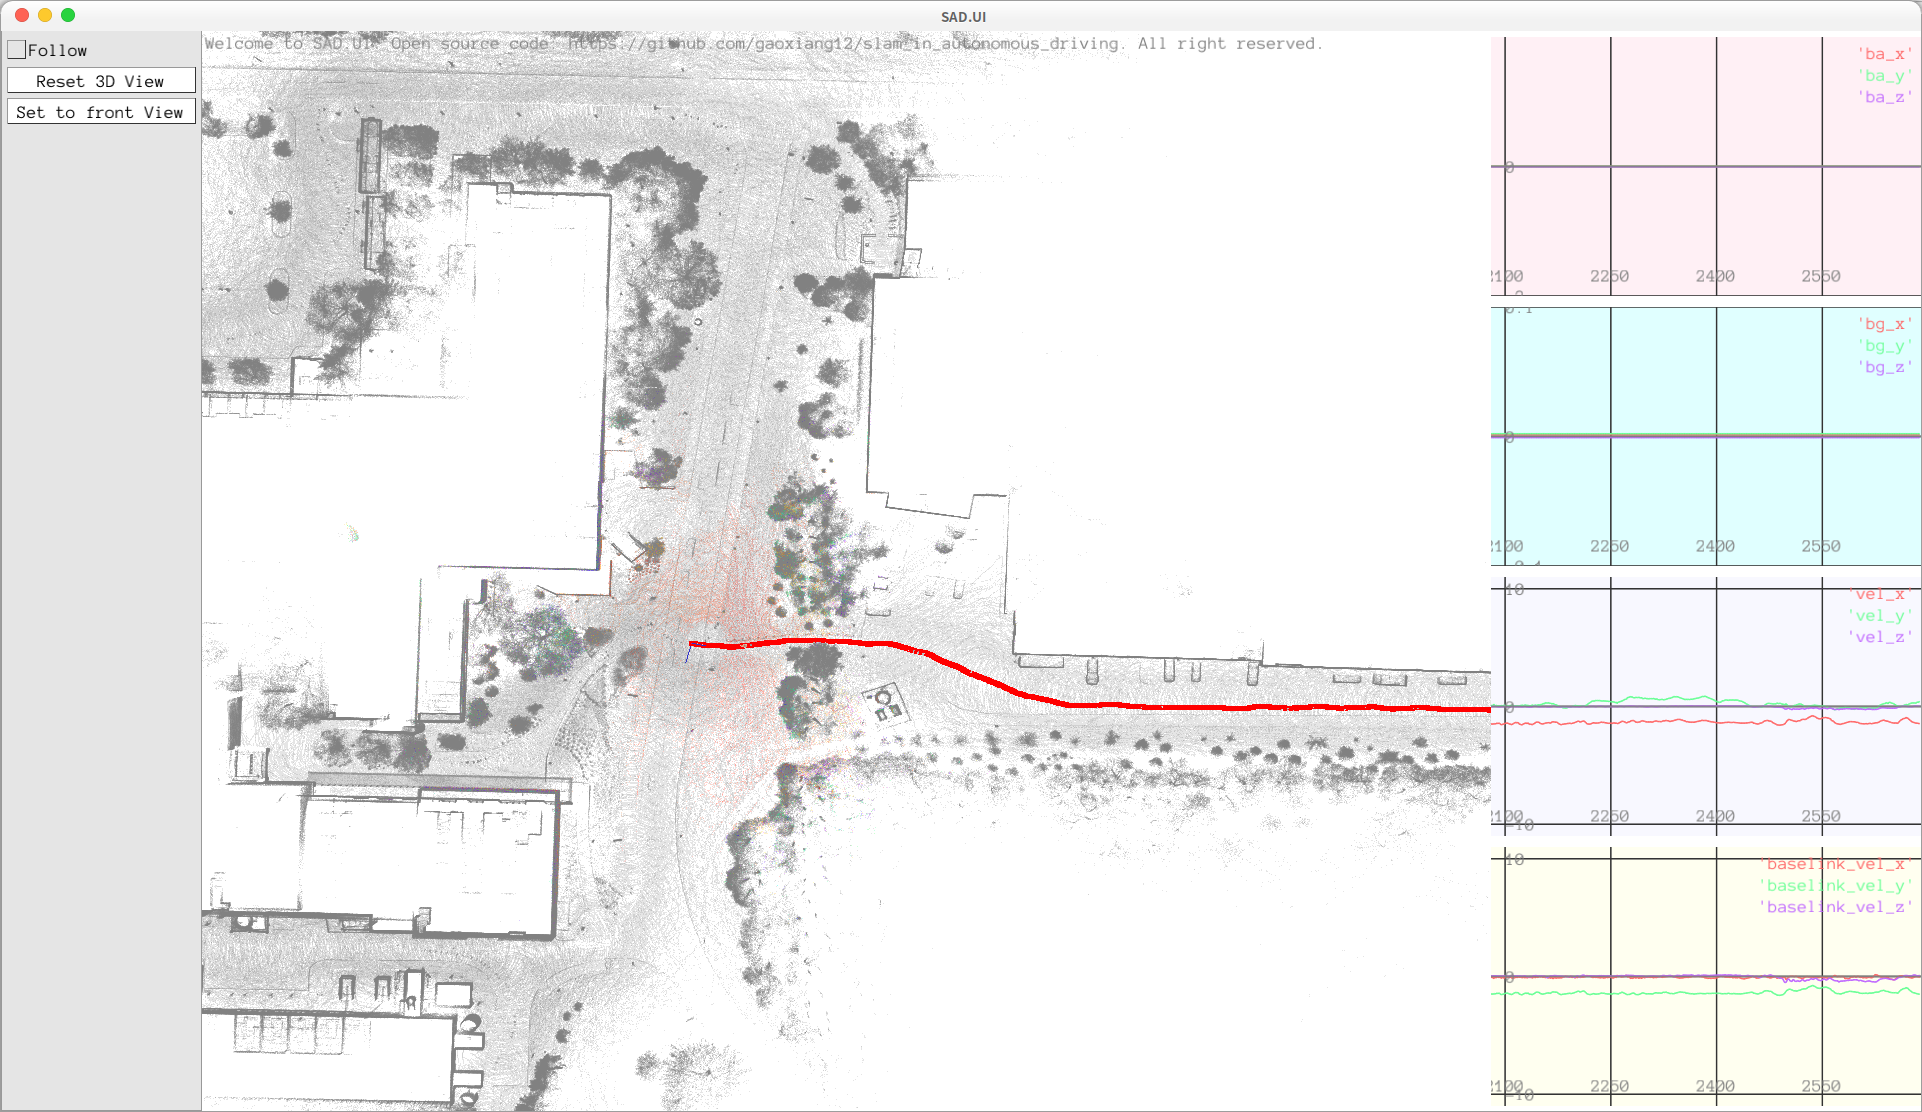
\includegraphics[width=1.0\textwidth]{resources/localization/fusion_offline.png}
	\caption{Test results of fusion localization}
	\label{fig:fusion-test}
\end{figure}

This section demonstrates the effectiveness of point cloud fusion localization. It shows that point cloud localization typically offers better robustness than RTK. As long as the point cloud map is sufficiently accurate, it can function effectively in most mapped areas without relying on outdoor RTK signal quality.

\begin{figure}[!t]
	\centering
	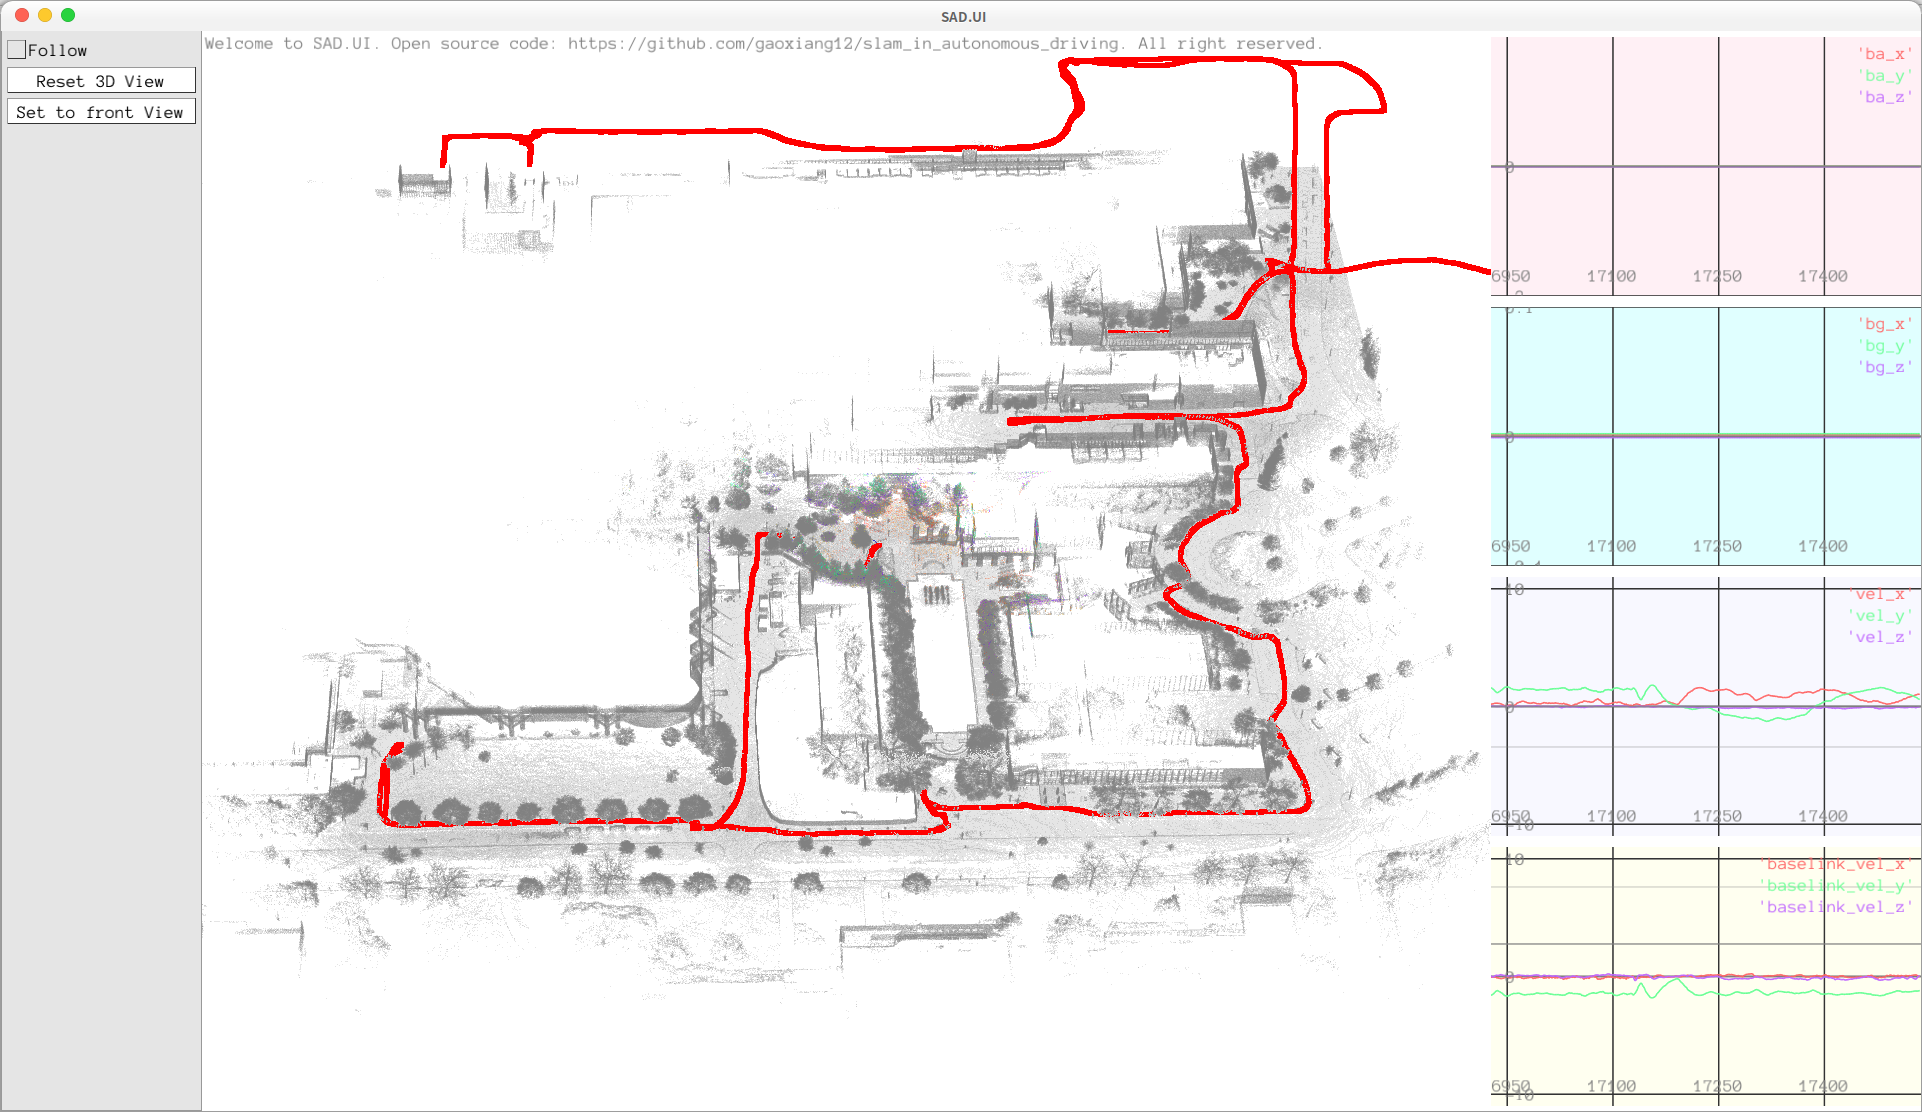
\includegraphics[width=1.0\textwidth]{resources/localization/fusion-full.png}
	\caption{Global results of fusion localization}
	\label{fig:fusion-loc}
\end{figure}

\section{Summary}
Building upon the point cloud mapping results from Chapter~\ref{cpt:mapping}, this chapter demonstrates a case study of fusion localization using existing LiDAR point cloud maps. The advantages and disadvantages of point cloud localization can be summarized as follows:

\begin{enumerate}
	\item Point cloud localization depends on scene structure rather than weather or occlusion conditions, typically offering better environmental adaptability than RTK. It works both indoors and outdoors with few limitations.
	\item Point cloud localization results can be integrated into ESKF filters like RTK or form an optimization system as in Chapter~\ref{cpt:preinteg}.
	\item For large-scale scenarios, the map should be partitioned, loading only nearby regions for localization.
	\item Unlike RTK, point cloud localization requires an initial approximate position. Insufficient initial accuracy may necessitate grid searches of nearby positions and angles.
	\item It shows some adaptability to dynamic scenes. As long as major structures (typically buildings) remain unchanged, small dynamic objects (crowds, vehicles, etc.) usually don't significantly interfere.
	\item For open areas, point cloud maps can be compressed into 2.5D maps \cite{Wolcott2017,Wolcott2015,Wan2018}, greatly reducing storage requirements. Due to space constraints, these compression algorithms aren't detailed here. Readers may refer to the literature for implementation details.
\end{enumerate}

\section*{Exercises}
\begin{enumerate}
	\item Test mapping and localization on other datasets provided with this book.
	\item Implement your own NDT to replace PCL's NDT, addressing lag during map transitions.
	\item Use NDT scores to evaluate matching quality, reinitializing the system when scores are too low.
	\item Adapt this program into a ROS node running via subscription callbacks (requires basic ROS knowledge).
	\item Experiment with compressing point cloud maps for 2D/2.5D map-based localization \cite{Wolcott2017}.
\end{enumerate}



